\chapter{Topic: Menger's sponge}
{ }\hfill\textbf{Level:} Advanced\\ \\
In this chapter, we're going to build a fractal solid called Menger's sponge. Here are the first steps to create this solid:
\begin{center}
\begin{minipage}{6cm}
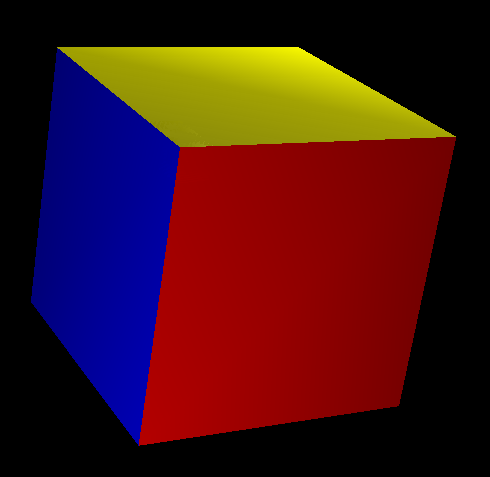
\includegraphics[width=6cm]{pics/menger0.png}
\begin{center}
 \textbf{Step 0}
\end{center}
\end{minipage}
\begin{minipage}{6cm}
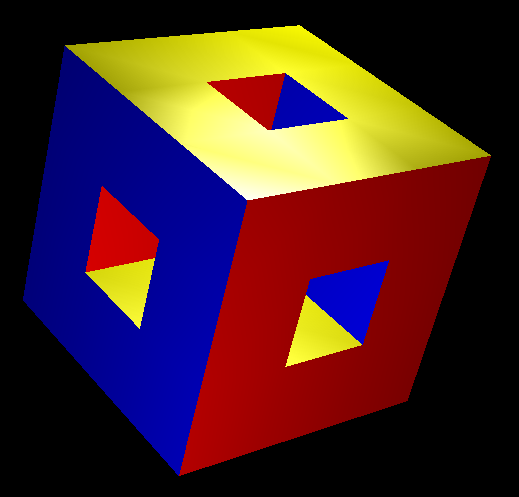
\includegraphics[width=6cm]{pics/menger1.png}
\begin{center}
 \textbf{Step 1}
\end{center}
\end{minipage}
\\
\begin{minipage}{6cm}
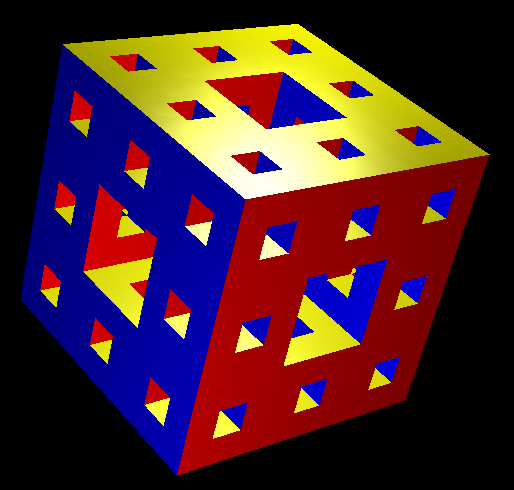
\includegraphics[width=6cm]{pics/menger2.png}
\begin{center}
 \textbf{Step 2}
\end{center}
\end{minipage}
\begin{minipage}{6cm}
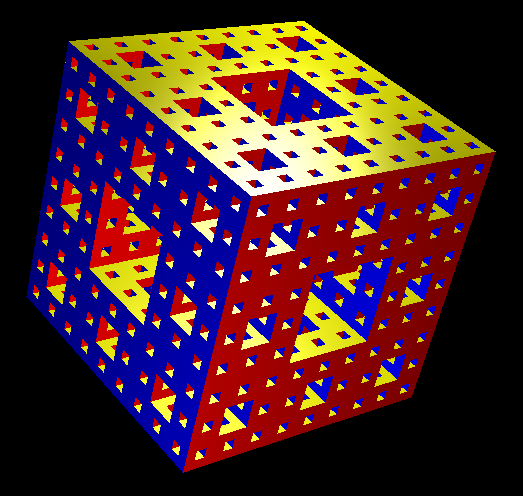
\includegraphics[width=6cm]{pics/menger3.png}
\begin{center}
 \textbf{Step 3}
\end{center}
\end{minipage}
\end{center}
This chapter contains two sections:
\begin{itemize}
 \item First, we'll show how to create this solid using recursion.
 \item Finally, we'll try to generate a Menger sponge of order~4.
\end{itemize}
\section{Using recursion}
\noindent Let's consider a Menger sponge of order $n$ which side length is $L$.\\
\begin{center}
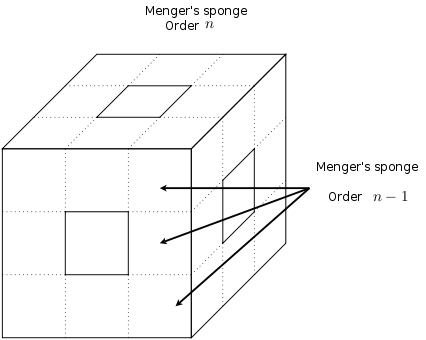
\includegraphics{pics/menger-schema01.png}
\end{center}
On the schema, we can see that this sponge contains 20 Menger sponges of order $n-1$ and with a side length $\dfrac{L}{3}$. The recursive structure of the sponge is well shown.\\ \\
\textbf{The program:}
\begin{verbatim}
to cube :l
if :counter=10000 [view3d]
# faces colors
localmake "colors [yellow magenta cyan blue]
# lateral faces
repeat 4 [setpencolor run item repcount :colors square :l right 90 forward  :l left 90 rightroll 90]
# bottom
setpencolor red downpitch 90 square :l uppitch 90
forward :l downpitch 90 setpencolor green square :l uppitch 90 back :l
end

to square :c
globalmake "counter :counter+1
polystart
repeat 4 [forward :c right 90]
polyend
end

# Menger's sponge
# p: recursion order
# l: side length of the cube
to menger :l :p
if :p=0 [cube :l] [
  localmake "p :p-1  
  localmake "l :l/3
  #front face
  repeat 3 [menger :l :p forward :l] back 3*:l
  right 90 forward :l left 90
  menger :l :p forward 2*:l menger :l :p back 2*:l
  right 90 forward :l left 90
  repeat 3 [menger :l :p forward :l] back 3*:l
  #right face 
 downpitch 90 forward :l uppitch 90 
  menger :l :p  forward 2*:l menger :l :p back 2*:l
  downpitch 90 forward :l uppitch 90 
  repeat 3 [menger :l :p forward :l] back 3*:l
  left 90 forward :l right 90
  menger :l :p  forward 2*:l menger :l :p back 2*:l
  left 90 forward :l right 90
  repeat 3 [menger :l :p forward :l] back 3*:l
  downpitch 90 back :l uppitch 90
  menger :l :p  forward 2*:l menger :l :p back 2*:l
   downpitch 90 back :l uppitch 90
]
end

to sponge :p
clearscreen hideturtle globalmake "counter 0 3d setscreencolor 0 menger 800 :p 
write [nombre penpaint polygone: ] print :counter 
view3d
end
\end{verbatim}
This program has four procedures:
\begin{itemize}
 \item \texttt{square :c}\\
This procedure draws a square which has side length \texttt{:c}. This polygon is stored in the 3D Viewer. The variable \texttt{counter} counts the number of drawn polygons.
 \item \texttt{cube :l}\\
This procedure draws a cube which has side length \texttt{:l}. Of course, it uses procedure \texttt{square}
 \item \texttt{menger :l :p}\\
This is the most important procedure of the program, it draws a Menger motif of order $p$ and with a side length equal to $l$. This motif is created using recursion as we have seen before on the schema.
 \item \texttt{sponge :p}\\
This procedure creates a Menger sponge, order $p$ with a side length equal to 800 and draws it in the Viewer 3D.
\end{itemize}
\vfill
\pagebreak
\section{Second approach: Drawing a Menger sponge, order 4}
The main advantage of the previous program is to exploit the recursive structure of the solid. This method is quite similar to the one we used to draw the Van Koch snowflake on p.\pageref{vankoch}. The main advantage of using recursion is a quite natural short program code. The disadvantage of the recursive approach is the number of created polygons: for example, a sponge of order 3 needs 48 000 polygons. \xlogo\ requires in this case an internal memory set to 256 Mb in the Preferences panel to prevent from memory overflow. \\ \\
If we want to draw a Menger sponge, order 4, we have to rethink the program and to forget recursion. We're going to create in this section a program that will draw the Menger solid of order 0,1,2,3 or 4.
\subsection{Sierpinski carpet}
\noindent Menger's sponge is the generalization in 3 dimensions of a plane figure called ``the Sierpinski carpet''. Here are the first steps to generate this figure:\\ \\
\begin{minipage}{4.5cm}
\begin{center}
 
\includegraphics[width=4.5cm]{pics/carpet0.png}\\
\textbf{Step 0}
\end{center}
\end{minipage}
\begin{minipage}{4.5cm}
\begin{center}
 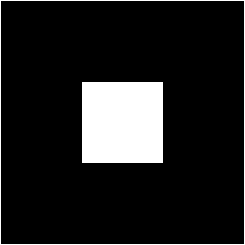
\includegraphics[width=4.5cm]{pics/carpet1.png}\\
\textbf{Step 1}
\end{center}
\end{minipage}
\begin{minipage}{4.5cm}
\begin{center}
 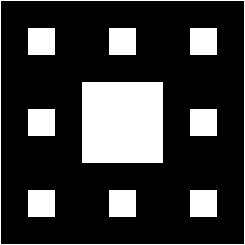
\includegraphics[width=4.5cm]{pics/carpet2.png}\\
\textbf{Step 2}
\end{center}
\end{minipage}
\begin{minipage}{4.5cm}
\begin{center}
 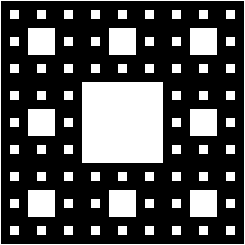
\includegraphics[width=4.5cm]{pics/carpet3.png}\\
\textbf{Step 3}
\end{center}
\end{minipage}\\ 
\vspace*{0.5cm}\\
Each face of a Menger sponge of order $p$ is a Sierpinski carpet of order $p$.
\subsection{Drawing a Sierpinski carpet of order $p$}
The objective is to set minimal the number of polygon to draw a Sierpinski carpet. The following example explains how to draw a Sierpinski carpet of order 3. Here, the first square has $3^3=27$ lines and 27 columns. We write in 3-basis each line number and each column number.
\begin{itemize}
 \item [\textbullet]\textbf{First step:} For each line whose number doesn't contain any 1, we draw a 27 units line. Using symmetry, we repeat the same operation on columns.\\
\begin{center}
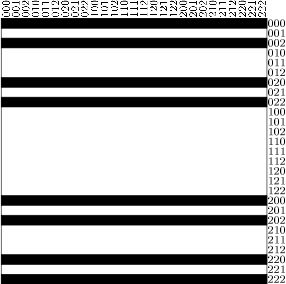
\includegraphics{pics/menger-schema02.png}
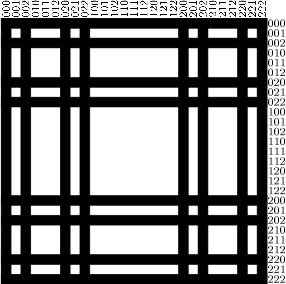
\includegraphics{pics/menger-schema03.png}
\end{center}
\vspace{0.2cm}
\item [\textbullet] \textbf{Second step:} Now, we're looking at lines whose numbers have a single 1 in first place. We draw rectangles of 9 units length by alternation.\\
\begin{center}
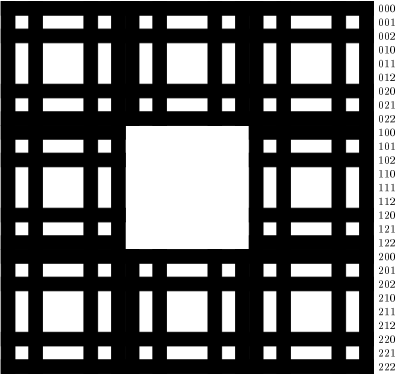
\includegraphics{pics/menger-schema04.png}
\end{center} 
\item [\textbullet] \textbf{Third step:} Now we're looking at lines whose number contains a single 1 in second place. We draw rectangles following the schema $[3\ 3\ 6\ 3\ 6\ 3\ 3]$. (It means 3 units pen down, 3 units pen up, 6 units pen down etc...). Using symmetry, we repeat this operation on columns.
\begin{center}
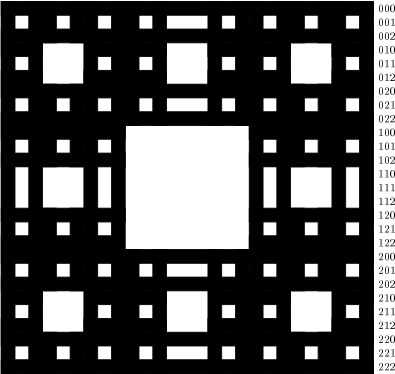
\includegraphics{pics/menger-schema05.png}
\end{center}
\item [\textbullet] \textbf{Final step:} Now we're looking at lines whose number contains a double 1 in the first two positions. We draw rectangles alternating following the schema $[3\ 3\ 3\ 9\ 3\ 3\ 3]$. We repeat this operation on columns.
\begin{center}
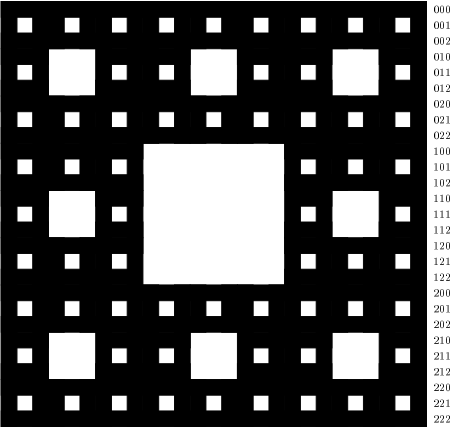
\includegraphics{pics/menger-schema06.png}
\end{center}
\end{itemize}
Now, we have built a Sierpnski carpet of order 3. To draw such a carpet, we need: $16+16+32+16=80$ polygons.
\subsection{All Different possible schemas for columns}
To recapitulate, here are the different column schemas according to the line numbers. (The symbol * represents 0 or 2)
\begin{center}
 \begin{tabular}{|c|c|}
 \hline
Number of line & Schema to apply \\
\hline
*** & 27 \\ 
\hline
1** &  9 9 9 \\
\hline
*1* & 3 3 6 3 6 3 3\\
\hline
11* & 3 3 3 9 3 3 3\\
\hline
\end{tabular}
\end{center}
In the same way, to build a carpet of order 4, we need a square with $3^4=81$ units. The line and column numbers will have 4 numbers in their writing in 3-basis. For each line number, here is the schema to apply (the symbol * represents 0 or 2):
\begin{center}
 \begin{tabular}{|c|c|}
 \hline
Line number & Schema to apply \\
\hline
 **** & 81 \\ 
\hline
1*** &  27 27 27 \\
\hline
*1** & 9 9 18 9 18 9 9 \\
\hline
**1* & 3 3 6 3 6 3 6 3 6 3 6 3 6 3 6 3 6 3 3 \\
\hline
*11* &  3 3 3 9 3 3 6 3 3 9 3 3 6 3 3 9 3 3 3 \\
\hline
1*1* & 3 3 6 3 6 3 3 27 3 3 6 3 6 3 3 \\
\hline
11** & 9 9 9 27 9 9 9 \\
\hline
111*& 3 3 3 9 3 3 3 27 3 3 3 9 3 3 3 \\
\hline
\end{tabular}\\
496 polygons are necessary to draw the a Sierpinski carpet of order 4.\\
\end{center}
Finally, here are the schema to apply for solid of order 2:
\begin{center}
  \begin{tabular}{|c|c|}
 \hline
Line numbers & Schema to apply\\
\hline
** &  9 \\
\hline
1* & 3 3 3 \\ 
\hline
\end{tabular}
\end{center}
\subsection{The program}
\begin{verbatim}
 # Draws a Sierpinski carpet of order :p and size :size
to carpet :size :p
globalmake "unit :size/(power 3 :p)
if :p=0 [ rec :size :size stop]
if :p=1 [repeat 4 [rec :size :unit forward :size right 90 ] stop]
for (list "x 1 power 3 :p) [
  localmake "cantorx cantor :x :p []
# We didn't draw elements with a 1 in last position
if  not (1=last :cantorx)  [
  localmake "nom evalue butlast :cantorx "
  drawcolumn :x getproperty "map :nom
  ]
]  
end

# output the writing in 3-basis of number x
# p order of the carpet (3^p units)
# :list empty list

to cantor :x :p :list
if :p=0 [output :list] 
localmake "a power 3 :p-1
if :x<= :a [
  output cantor  :x :p-1  sentence :list 0] 
  [ if :x<=2*:a [output cantor  :x-:a :p-1  sentence :list 1] 
  output cantor :x-2*:a :p-1 sentence :list 0]
end

# Draw the column number x respecting the schema in list :list
to drawcolumn :x :list
  penup  right 90 forward (:x-1)*:unit left 90  pendown des :list
  penup left 90 forward (:x-1)*:unit right 90 forward :x*:unit right 90 pendown des :list
penup left 90 back :x*:unit pendown
end

# Draws a rectangle with choosen dimensions
# It is stored in 3D viewer
to rec :lo :la
globalmake "compteur :compteur+1
polystart
repeat 2 [forward :lo right 90 forward :la right 90]
polyend
end

# Inits the different possible columns for carpet order 0 to 4
to initmap
putproperty "map 111 [3 3 3 9 3 3 3 27 3 3 3 9 3 3 3]
putproperty "map 110 [9 9 9 27 9 9 9]
putproperty "map 101 [3 3 6 3 6 3 3 27 3 3 6 3 6 3 3]
putproperty "map 011 [3 3 3 9 3 3 6 3 3 9 3 3 6 3 3 9 3 3 3]
putproperty "map 000 [81]
putproperty "map 100 [27 27 27]
putproperty "map 010 [9 9 18 9 18 9 9]
putproperty "map 001 [3 3 6 3 6 3 6 3 6 3 6 3 6 3 6 3 6 3 3]
putproperty "map 01 [3 3 6 3 6 3 3]
putproperty "map 00 [27]
putproperty "map 10 [9 9 9]
putproperty "map 11 [3 3 3 9 3 3 3]
putproperty "map 1 [3 3 3]
putproperty "map 0 [9]
end

# if the 3-basis writing is  [1 0 1] --> output 101
to evalue :list :mot
  if emptyp :list [output :mot]
  [
  localmake "mot word :mot first :list
  output evalue butfirst :list :mot  
]
end
# Draws the block of rectangles alternanting
to des :list
localmake "somme 0
for (list "i 1 count :list) [
   localmake "element item :i :list
    localmake "somme :element+:somme 
  if even? :i [penup forward :element*:unit pendown ] [rec :element*:unit :unit forward :element*:unit]  
]
penup back  :somme * :unit pendown
end

# Is this number even?
to pair? :i
output 0=reste :i 2
end

# Draws the carpet order :p
to tapis :p
clearscreen 3d hideturtle initmap
globalmake "compteur 0
carpet 810 :p
write "nombre\ de\ polygones:\  print :compteur 
view3d
end

# Is this number even?
to even? :i
output 0=modulo :i 2
end

\end{verbatim}
\texttt{tapis 3} draws a Sierpinski carpet of order 3 with a side length equal to 810. Here we are! Now we can come back to the Menger's sponge!
\subsection{Menger's sponge order 4}
The Menger sponge has a lot of symmetries. To build the sponge, we're going to draw the different sections along the plane $(xOy)$ and then repeat those figures along the planes $(yOz)$ and $(xOz)$. To explain what happens, let's have a look at the sponge of order 2:\\
When we cut with a vertical plane, we can obtain four different motifs:\\
 \begin{center}
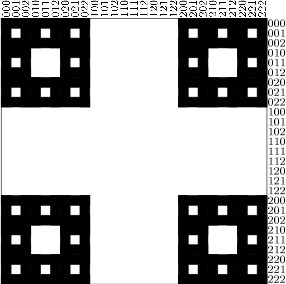
\includegraphics{pics/menger-schema07.png} \\ \vspace{1cm}
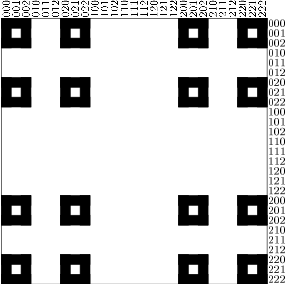
\includegraphics{pics/menger-schema08.png} \\ \vfill
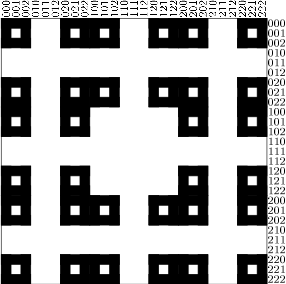
\includegraphics{pics/menger-schema09.png} \\ \vspace{1cm}
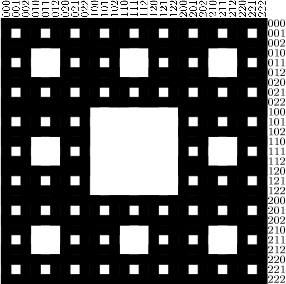
\includegraphics{pics/menger-schema10.png}\\ 
\end{center}
To draw a sponge of order 3, we're going to browse the number from 1 to 27, it means from 001 to 222 in 3 basis. For each number, we'll apply the valid section and we'll report this figure along $(Ox)$, $(Oy)$ and $(Oz)$.
\subsubsection{The code}
\noindent With this program, we can draw Menger's sponge of order 0,1,2,3 and 4.
\begin{verbatim}
 # Draws a Sierpinski carpet of order :p and size :size
to carpet :size :p
globalmake "unit :size/(power 3 :p)
if :p=0 [ rec :size :size stop]
if :p=1 [repeat 4 [rec :size :unit forward :size right 90 ] stop]
for (list "x 1 power 3 :p) [
  localmake "cantorx cantor :x :p []
# We didn't draw elements with a 1 in last position
if  not (1=last :cantorx)  [
  localmake "nom evalue butlast :cantorx "
  drawcolumn :x getproperty "map :nom
  ]
]  
end

# output the writing in 3-basis of number x
# p order of the carpet (3^p units)
# :list empty list

to cantor :x :p :list
if :p=0 [output :list] 
localmake "a power 3 :p-1
if :x<= :a [
  output cantor  :x :p-1  sentence :list 0] 
  [ if :x<=2*:a [output cantor  :x-:a :p-1  sentence :list 1] 
  output cantor :x-2*:a :p-1 sentence :list 2]
end

# Draw the column number x respecting the schema in list :list
to drawcolumn :x :list
  penup  right 90 forward (:x-1)*:unit left 90  pendown des :list
  penup left 90 forward (:x-1)*:unit right 90 forward :x*:unit right 90 pendown des :list
penup left 90 back :x*:unit pendown
end

# Draws a rectange with choosen dimensions
# It is stored in 3D viewer
to rec :lo :la
globalmake "counter :counter+1
polystart
repeat 2 [forward :lo right 90 forward :la right 90]
polyend
end

# Inits the different possible columns for carpet order 0 to 4
to initmap
putproperty "map 111 [3 3 3 9 3 3 3 27 3 3 3 9 3 3 3]
putproperty "map 110 [9 9 9 27 9 9 9]
putproperty "map 101 [3 3 6 3 6 3 3 27 3 3 6 3 6 3 3]
putproperty "map 011 [3 3 3 9 3 3 6 3 3 9 3 3 6 3 3 9 3 3 3]
putproperty "map 000 [81]
putproperty "map 100 [27 27 27]
putproperty "map 010 [9 9 18 9 18 9 9]
putproperty "map 001 [3 3 6 3 6 3 6 3 6 3 6 3 6 3 6 3 6 3 3]
putproperty "map 01 [3 3 6 3 6 3 3]
putproperty "map 00 [27]
putproperty "map 10 [9 9 9]
putproperty "map 11 [3 3 3 9 3 3 3]
putproperty "map 1 [3 3 3]
putproperty "map 0 [9]
end

# if the 3-basis writing is  [1 0 1] --> output 101
# if the 3-basis writing is [1 0 2] --> output 100
#  Element from the list are translated into a word. 
# 2 are replaced by 0

to evalue :list :mot
  if emptyp :list [output :mot]
  [
  localmake "first first :list
  if :first=2 [localmake "first 0] 
 localmake "mot word :mot :first
  output evalue butfirst :list :mot  
]
end
# Draws the block of rectangular alternanting
to des :list
localmake "somme 0
for (list "i 1 count :list) [
   localmake "element item :i :list
    localmake "somme :element+:somme 
  if even? :i [penup forward :element*:unit pendown ] 
      [rec :element*:unit :unit forward :element*:unit]  
]
penup back  :somme * :unit pendown
end

# Draws the carpet order :p
to tapis :p
clearscreen 3d hideturtle initmap
globalmake "compteur 0
carpet 810 :p
write "nombre\ de\ polygones:\  print :compteur 
view3d
end

# Is this number even?
to even? :i
output 0=modulo :i 2
end


# Remove the last 1 from :list
to deletelastone :list
for (list "i count :list 1 minus 1) [
  localmake "element item :i :list 
  if :element=1 [localmake "list replace :list :i 0 stop] [if :element=2 [stop]]
]
output :list
end

# Draws the Serpinski carpet 
# along axis (ox), (oy) and (oz)
to draw3carpet :size :order :z
penup home  
uppitch 90 forward (:z-1)*:unite downpitch 90 pendown
setpencolor blue run :order :size
penup home  
leftroll 90 forward (:z-1)*:unite downpitch 90  pendown
setpencolor yellow run :order :size
penup home  
uppitch 90 forward :size right 90 forward (:z-1)*:unite downpitch 90 pendown
setpencolor magenta run :order :size 
end

# Menger's sponge order :p and size :size

to menger :size :p
globalmake "unite :size/(power 3 :p)
for (list "z 1 power 3 :p) [
  localmake "cantorz cantor :z :p []
  localmake "last last :cantorz
  localmake "cantorz butlast :cantorz
  if :last=0 [localmake "order evalue deletelastone :cantorz "] 
           [localmake "order evalue :cantorz "]
  localmake "order word "coupe :order
  draw3carpet :size :order :z
  penup uppitch 90 forward :unit downpitch 90 pendown 
]
draw3carpet :size :order (power 3 :p)+1
end


# Main procedure
# Draws a sponge order :p with side length 405
to sponge :p
clearscreen setsc 0 3d hideturtle
localmake "time pasttime
initmap
globalmake "counter 0
if :p=0 [cube 405] [menger 405 :p]
# Displays the time to build the sponge
write "Polygons\ number:\  print :counter 
write "Time:\  print pasttime -:time 
view3d
end

# Different sections for menger order 2
to coupe1 :size
repeat 4 [carpet :size/3 1 penup forward :size right 90 pendown]
end

to coupe0 :size
carpet :size 2
end

# Different sections for Menger order 3

to coupe10 :size
repeat 4 [carpet :size/3 2 penup forward :size right 90 pendown]
end

to coupe01 :size
repeat 4 [repeat 2 [coupe1 :size/3 penup forward :size/3 pendown] forward :size/3 right 90]
end

to coupe11 :size
repeat 4 [coupe1 :size/3 penup forward :size right 90 pendown]
end


to coupe00 :size
carpet :size 3
end

# Different sections for Menger order 4
to coupe000 :size
carpet :size 4
end

to coupe100 :size
repeat 4 [carpet :size/3 3 penup forward :size right 90 pendown]
end

to coupe010 :size
repeat 4 [repeat 2 [coupe10 :size/3 penup forward :size/3 pendown] forward :size/3 right 90]
end

to coupe001 :size
repeat 4 [repeat 2 [coupe01 :size/3 penup forward :size/3 pendown] forward :size/3 right 90]
end

to coupe110 :size
repeat 4 [coupe10 :size/3 penup forward :size pendown right 90 ]
end

to coupe111 :size
repeat 4 [coupe11 :size/3 penup forward :size right 90 pendown]
end

to coupe101 :size
repeat 4 [coupe01 :size/3 penup forward :size right 90 pendown]
end

to coupe011 :size
repeat 4 [repeat 2 [coupe11 :size/3 penup forward :size/3 pendown] forward :size/3 right 90]
end

to coupe :size
carpet :size 1
end

to cube :size
repeat 2 [
setpencolor blue rec :size :size penup forward :size downpitch 90 pendown 
setpencolor yellow rec :size :size penup forward :size downpitch 90  pendown
]
setpencolor magenta
penup leftroll 90 left 90 forward :size right 90 pendown rec :size :size
penup right 90 forward :size left 90 rightroll 90 right 90 forward :size left 90 rightroll 90 pendown rec :size  :size
leftroll 90 left 90 forward :size right 90
end
\end{verbatim}
Then, we set memory allocated to \xlogo\ to 640 Mb: \texttt{sponge 4}
\begin{center}
 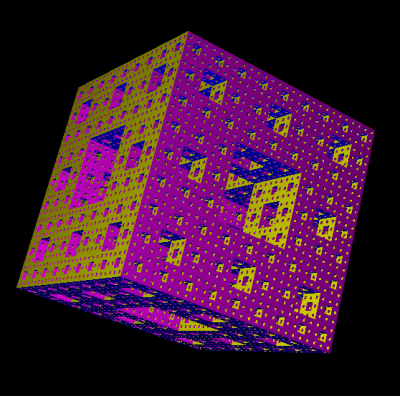
\includegraphics{pics/menger-menger4.png}
\end{center}